\documentclass{article}
\usepackage[utf8]{inputenc}
\usepackage{subfig}

%References
\usepackage{natbib}
%IMPORTANT use https://www.citationmachine.net/ if you need to generate references!
% \citep{reference} creates Harvard Style references throughout

%Colors
\usepackage{xcolor}

\usepackage[protrusion=true,expansion]{microtype}

%Code Markup
\usepackage[outputdir=cache]{minted}
%Syntax Highlighting Style
\definecolor{bggray}{RGB}{40,40,40}
\newmintedfile[javacode]{java}{
	style=fruity,
	bgcolor=bggray,
	linenos,
	breaklines,
	tabsize=2,
	obeytabs
}

%Page Margins and stuff
\usepackage{geometry}
 \geometry{
 a4paper,
 total={170mm,257mm},
 left=20mm,
 }

%Pictures
\usepackage{graphicx}
\graphicspath{ {./images/} }

%Move the title position
\usepackage{titling}

\setlength{\droptitle}{-8.5em} %Up, near the top but not too high

\title{Assignment 3 - CT2106 Object Oriented Programming}
\author{Daniel Hannon (19484286)}
\date{November 2020}

\begin{document}
	\maketitle
	\section{Description}
	With this Assignment, we had to use class inheritance to create four different animal types, each with several unique features. As they were all child classes of the parent class \textbf{Animal} they could all be stored in an array as they all had some common traits. 
	\section{Code}
	\subsection{AnimalTest}
	\javacode{Animaltester.java}
	\subsubsection{AnimalTest outputs}
	\begin{figure}[h!]
		\centering
		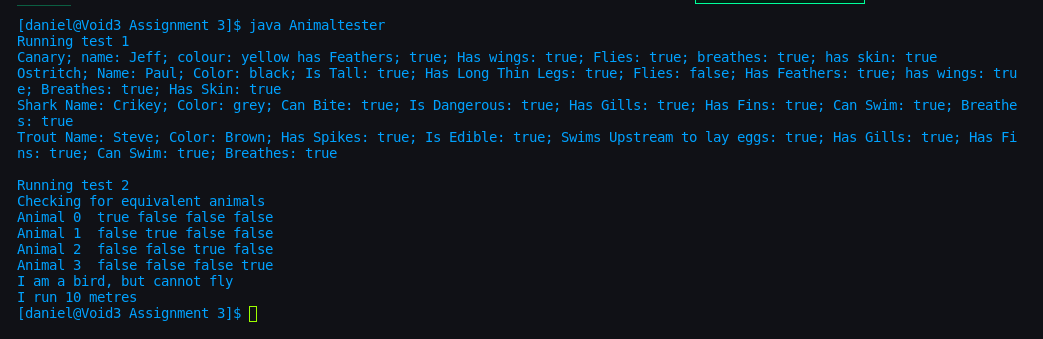
\includegraphics[width=\textwidth]{outputs.png}
	\end{figure}
	\subsection{Canary}
	\javacode{Canary.java}
	\subsection{Ostritch}
	\javacode{Ostritch.java}
	\subsection{Fish}
	\javacode{Fish.java}
	\subsection{Shark}
	\javacode{Shark.java}
	\subsection{Trout}
	\javacode{Trout.java}
	\section{Code Explanation}
	The Code is fairly straightforward, the \textbf{toString()} overwrites all return every feature of the animal in string format as specified.\\
	The \textbf{equals(Object o)} uses the Equals property of the \textbf{String} type as if the objects are equal, their strings are equivalent. But in order to prevent passing a \textbf{String} type into \textbf{equals{Object o}} they perform a sense check by attempting to typecast the \textbf{Object} passed into the method. This is wrapped in a \textbf{try/catch} and returns false if the object passed is not of the same type. \\
	I reused this method for every Animal class as it is very versatile and it verifies that the \textbf{toString()} overwrite works for each Object class.\\
	There is a distinct lack of setters as a most if not all of the characteristics of the animals do not change during its life, unless the animal is dead but that is out of scope. \\
	Ostritches output \textbf{\textit{I am a bird but I cannot fly}} by the addition of an if/else in the parent \textbf{Bird} class.
	%Sets to Harvard Style and links the references file
	\bibliographystyle{agsm}
	\bibliography{references}
\end{document}